\documentclass[12pt]{article}
\usepackage{fullpage,enumitem,amsmath,amssymb,graphicx, listings,cite}%,hyperref}

\usepackage{hyperref}
\usepackage{xcolor}
\usepackage{subcaption}

\hypersetup{
   colorlinks,
   linkcolor={red!50!black},
   citecolor={blue!50!black},
   urlcolor={blue!80!black}
}

\title{Enabling Affordable Precision Agriculture by Sensing Soil Moisture Wirelessly}
\author{Colleen Josephson\\Advised by:  Ranveer Chandra (Microsoft) and Sachin Katti (Stanford)\\\textbf{Do not forward}}

\begin{document}
\maketitle

\begin{abstract}
  The term ``precision agriculture'' has been around since the 1980s,
  and it describes a farming technique that uses extensive measurement
  of crop data to make informed decisions about watering,
  fertilization and more. Despite decades of work, precision
  agriculture is still not widely implemented on working farms. This
  is because the data is hard to collect and process, primarily due to
  the lack of high speed internet access in rural areas, and the high
  cost and difficulty of deploying dense sensor networks. Recent work
  such as Farmbeats~\cite{farmbeats} has made good progress in
  addressing the issues of internet access, but the cost and
  deployability of sensors remains an issue. We seek to address this
  by designing a low-cost and easy-to-use wireless soil moisture
  sensor.
\end{abstract}


\section*{Introduction}

Agriculture is the single largest pressure on the world's sources of
fresh water--- 69\% of the global fresh water supply is used for
agriculture~\cite{water}. Paired with the fact that the world's
population is projected to exceed 9 billion by 2050~\cite{population},
with most of the growth coming from developing nations in Africa,
conservation of fresh water and sufficient food production are key
concerns that need to be addressed. Soil moisture is the most
important measurement for ensuring the maximization of crop yield
without water waste.

Multiple studies show that soil moisture sensors lead to a water
savings of at least 20\%\cite{watersavings}, and in some cases more
than 50\%, while maintaining crop yields. Yet soil sensors are still
not widely deployed on working farms, despite decades of research
confirming the benefits. The lack of widespread adoption can be
attributed to a few key challenges: 1.) high sensor cost 2.)
difficulty of deploying and maintaining the sensors and 3.) difficulty
collecting and processing the sensor data.

The average commercial\footnote{People are often misled by the
  SparkFun soil moisture sensor retailing for \$6.95. This is just a
  raw sensor probe, with no wiring, weatherproofing, testing or
  calibration. The added cost of a power source, data logger and
  wiring is more than \$40, and the system is still not weatherproofed
  or calibrated.} soil moisture sensor is more than \$100, which does
not include the power source or data logger to record and/or transmit
the measurement samples. The cost is at least \$50 to add the cheapest
DIY weatherproof logger and transmitter.  Since soil is not uniform
across a field, nevermind an entire farm, multiple sensors are needed
to accurately measure moisture for irrigation purposes. The average
farm in the United States is 444 acres~\cite{farmsize}. The water cost
for a tomato farm of that size would be approximately \$55,000 per
year~\cite{agwater}~\cite{tomatoes}, which means a precision soil
moisture system would lead to \$11,000 in savings. However, the cost
of deploying 20 sensors~\cite{sensorDensity} per acre would more than
\$1,000,000 with today's sensor costs. The current high cost of
sensors makes it difficult to for the average farmer to justify
investing in precision agriculture. Furthermore, this cost makes soil
moisture sensing completely infeasible for small-holder farmers in
developing nations, which is where the most of the food and water
insecurity will be located.

On top of the high cost, current sensors are not simple to deploy and
maintain. Very few sellers offer a product that includes the sensor,
logger and power source ready for immediate use. Therefore some amount
of setup labor is required for each sensor. Figure 1 shows a typical
sensor and data logging system. Though the sensor is waterproof, the
data logger (in this case an Arduino) needs to be waterproofed and
powered. The soil moisture sensor needs to be buried, which requires
digging a hole to the desired depth. This project also attaches solar
panel to the battery pack, which requires mounting high enough to
harvest sunlight, probably requiring a wooden or metal post. The
laborious process of burying the sensor and mounting the solar panel
would need to be repeated for every sensor node on the
farm. Furthermore, the excess cables and bulky box also make the
system easy to tangle in farm equipment and tools. The sensor system
would need to gently removed and re-deployed every time the field is
tilled. This all adds up to a significant amount of manual labor to
deploy and maintain the soil moisture sensors.

\begin{figure*}[h!]
  \centering
  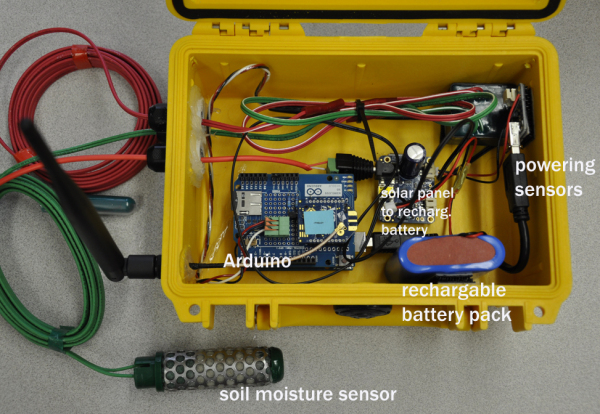
\includegraphics[scale=0.75]{soil_moisture_sn_setup.jpg}\\
  \caption{A weatherproofed soil moisture sensor box from the
    Geosensor Networks Lab~\cite{sensorbox}}
\end{figure*}

Finally, the data needs to be collected from the logger. For a 444
acre farm, the most practical method is wireless collection. Extending
wireless coverage to a large farm is not simple, especially because
cellular coverage in rural areas tends to be poor. A number of recent
works have considered the issue of networking sensors in rural
environments. For example, the 2015 Farmbeats project looks at the
issue of sensor data collection and network access extensively, using
TV whitespace technology to provide a wireless gateway from the field
to the Internet. Though solving this challenge is also important, the
focus of our research will be on reducing the cost and improving the
deployability and maintainability of soil moisture sensors.

In the next section we will give an overview of current sensing
technology and related work.

\section*{Overview of sensing techniques}

The most accurate way to measure soil moisture is gravimetrically,
where a soil sample is taken, weighed, allowed to dry (by oven or
otherwise) and re-weighed~\cite{Noborio2001}. This process is
time-intensive and requires physical removal of soil at the depth you
wish to measure, so it is impractical for irrigation purposes. There
are three primary types of practical soil moisture sensors used in
agriculture: tensiometers, resistive sensors, and volumetric
sensors~\cite{sensorTypes}.

\subsubsection*{Tensiometers} Tensiometers measure soil water
tension. An air-free tube of water is attached to a porous tip, such as
ceramic. As water extracted from the soil by plants, the vacuum in the
tube increases. When the soil is irrigated, the pressure decreases. A
pressure sensor at the top of the tube is used to make the moisture
measurements. The response time to moisture changes is typically 2-3
hours. Tensiometers are slightly cheaper than the volumetric sensors
discussed earlier, but still require a dedicated data
logger/transmitter. They typically require regular maintenance, such as
adding water or removing air from the tube. Tensiometers also only
operate when soils are relatively wet, and cannot be used when there
is any risk of freezing temperatures.

\subsubsection*{Resistive sensors}
Resistive sensors are among the cheapest sensors. These sensors have
two probes in the soil and current passes through the soil between the
probes. The moisture value is determined by measuring the
resistance. DIY soil moisture kits, like the SparkFun~\cite{sparkfun}
sensor, are usually resistive. Resistance-based sensors are the least
accurate, and the probes corrode quickly~\cite{capVSres}. Granular
matrix sensors (GMS) are a variation on resistive sensors. They
measure electrical resistance in a porous medium like ceramic. As
water seeps into the porous medium, it reduces the electrical
resistance. The ceramic in GMSes prevents probe decay and naturally
filter out ions from fertilizer and salt, which improves the accuracy
of the readings. GMSes cost similar to tensiometers, but take longer
to respond, do not work well in very wet soil, and are more difficult
to install. They do, however, require significantly less maintenance.

\subsubsection*{Volumetric sensors}Volumetric sensors estimate
$\frac{V_{water}}{V_{wet soil}}$, the ratio of the volume of the water
to the volume of the soil plus the same volume of water. As the
volumetric water content changes, the dielectric permittivity constant
of the soil changes. Recall that dielectric permittivity,
$\varepsilon$, is the ability of a substance to hold an electrical
charge. The dielectric permittivity constant (also known as relative
permittivity), $\varepsilon_r$, is the ratio of the permittivity of
the substance to the permittivity of free space,
$\varepsilon_0$. Permittivity is often treated as a complex number:
$\varepsilon = \varepsilon' + j\varepsilon ''$, where $\varepsilon '$
is the real component and $\varepsilon''$ is the complex.

There are two main types of volumetric sensors: capacitive and time
domain refelectometry (TDR). Capacitive sensors measure the charge
time of a capacitor, which is a roughly linear function of
$\varepsilon$~\cite{sensorOverview}. Capacitive sensors are much less
prone to corrosion than resistive sensors, and are more accurate. For
this reason, capacitive sensors are available as commercial-grade soil
moisture sensors. 

Time domain reflectometry (TDR) is another common method for measuring
soil moisture that takes advantage of the frequency dependence of the
dielectric permittivity. It measures the propagation time of EM waves
by sending a pulse down a cable and into the soil probe and measuring
how long it takes before the signal is reflected and returns. We call
this the \emph{time of flight}, or ToF. This method of soil moisture
measurement generates wideband signals (100Mhz-3Ghz for agricultural
grade) to ensure sufficient time resolution. Like capacitive sensors,
the probes must maintain good contact with the soil for accurate
measurements. The cost of a sensor is about \$1000.

A related technique uses ground penetrating radar (GPR) to calculate
the time of flight. GPR is also wideband and costs thousands of
dollars. Generally the equipment is large (~the size of a lawnmower)
and needs to be dragged across the surface of the soil. This is a
labor intensive process which may not always be possible in dense
crops. Non-contact GPRs exist that can be attached to drones, but
these have lower resolution and can only reliably measure to a depth
of about 10cm~\cite{gprEdaphic}.

\subsubsection*{Novel soil moisture sensors}
A number of recent efforts have explored ways to lower the cost of
soil moisture sensors. \cite{Hasan2013} and uses passive RFID tags to sense
impedance changes caused by soil moisture, but their system requires a
\$1000+ RFID reader, a free-air reference tag, and a delicate antenna
needs to remain on the surface of the soil in order to collect the
readings. \cite{Dey2016} measures the shift in resonance frequency of the
scattering parameter (S-parameter). Their technique required the use
of a vector network analyzer (VNA), so it would require a potentially
costly custom reader. Both of the above approaches were only tested in
an indoors laboratory environment, and they do not provide any
comparisons to the 'ground truth' or an existing commercial sensor.

\cite{Daskalakis2016} attaches a capacitive sensor to an above-ground dipole
antenna. The readings are collected using a low-cost software defined
reader. The authors claim a cost of 6 Euro, which is the lowest-cost
sensor that was actually deployed. However, this cost is without any
weatherproofing, and a key tradeoff is a 4x decrease in resolution
over commercial sensors.


In 2017 researchers at Microsoft Research figured out how to measure
soil moisture using consumer-grade WiFi signals. This system, called
SMURF~\cite{smurf}, uses time of flight like TDR and GPR. However, in
order to use the relatively narrow bandwidth of WiFi it relies on the
\emph{relative} time of flight, which is the difference in time of
arrival between antennas in a MIMO system. The system is still
difficult to deploy and maintain because it requires burying multiple
WiFi antennas in the ground and connecting them via cable to an active
receiver such as an Atheros WiFi card. Then, a different active
transmitter must send packets to the antennas in the ground in order
to collect the measurements. The antennas are not as sensitive to soil
contact as TDR and capacitive sensors, but the soil packing between
antennas impacts the measurements. While SMURF is an important
stepping stone, this work is impractical for deploying at-scale on a
farm.

\section*{Proposed approach}
How can we take the low-cost of SMURF and make it practical to deploy
and use? The extremely low cost of backscatter tags (such as RFID) make
it an attractive option to explore. Passive RFID tags can be purchased
for as little as 7 cents~\cite{rfidcost}. The need to use a
proprietary reader is eliminated with WiFi backscatter tags
like~\cite{Zhang2017}~\cite{Zhang2016}. When the cost of the sensors
is so low, the system becomes more maintainable because it is
inexpensive to replace failing or broken sensors. Furthermore, the
small form factor of backscatter tags makes them easier to embed in
the soil, which makes it possible to take measurements at multiple
depths per sensor site. It also opens up opportunities for novel
deployment systems, such as attaching the tags to a soil auger.

The same relative time of flight approach cannot be used, though,
since the power savings and low cost of backscatter tags comes from
the lack of an active receiver. Calculating accurate ToF from
commodity WiFi devices is very difficult~\cite{Vasisht2015}, which is
why SMURF uses relative ToF. It is potentially possible for a MIMO
receiver to separate signals from multiple tags using the MUSIC
algorithm~\cite{Soltanaghaei2018}~\cite{Kotaru2015} and calculate the
ToF delta between the multiple reflections, but significant challenges
still remain to to get enough signal strength from the buried
backscatter devices.

WiFi is attractive because of its ubiquity and low cost, but
consumer-grade RADAR systems are becoming increasingly affordable and
accessible, which introduces exciting new sensing possibilities. There
are multiple radar devices on the market compatible with Android
phones~\cite{walabot}~\cite{omnipresense}, ranging from \$50-200. On their own,
consumer-grade radar systems are incapable of sensing soil
moisture---that would require the still-expensive technology of ground
penetrating radar. These cheap radars, however, could be paired with
backscatter tags.

\begin{figure*}[h!]
  \centering
  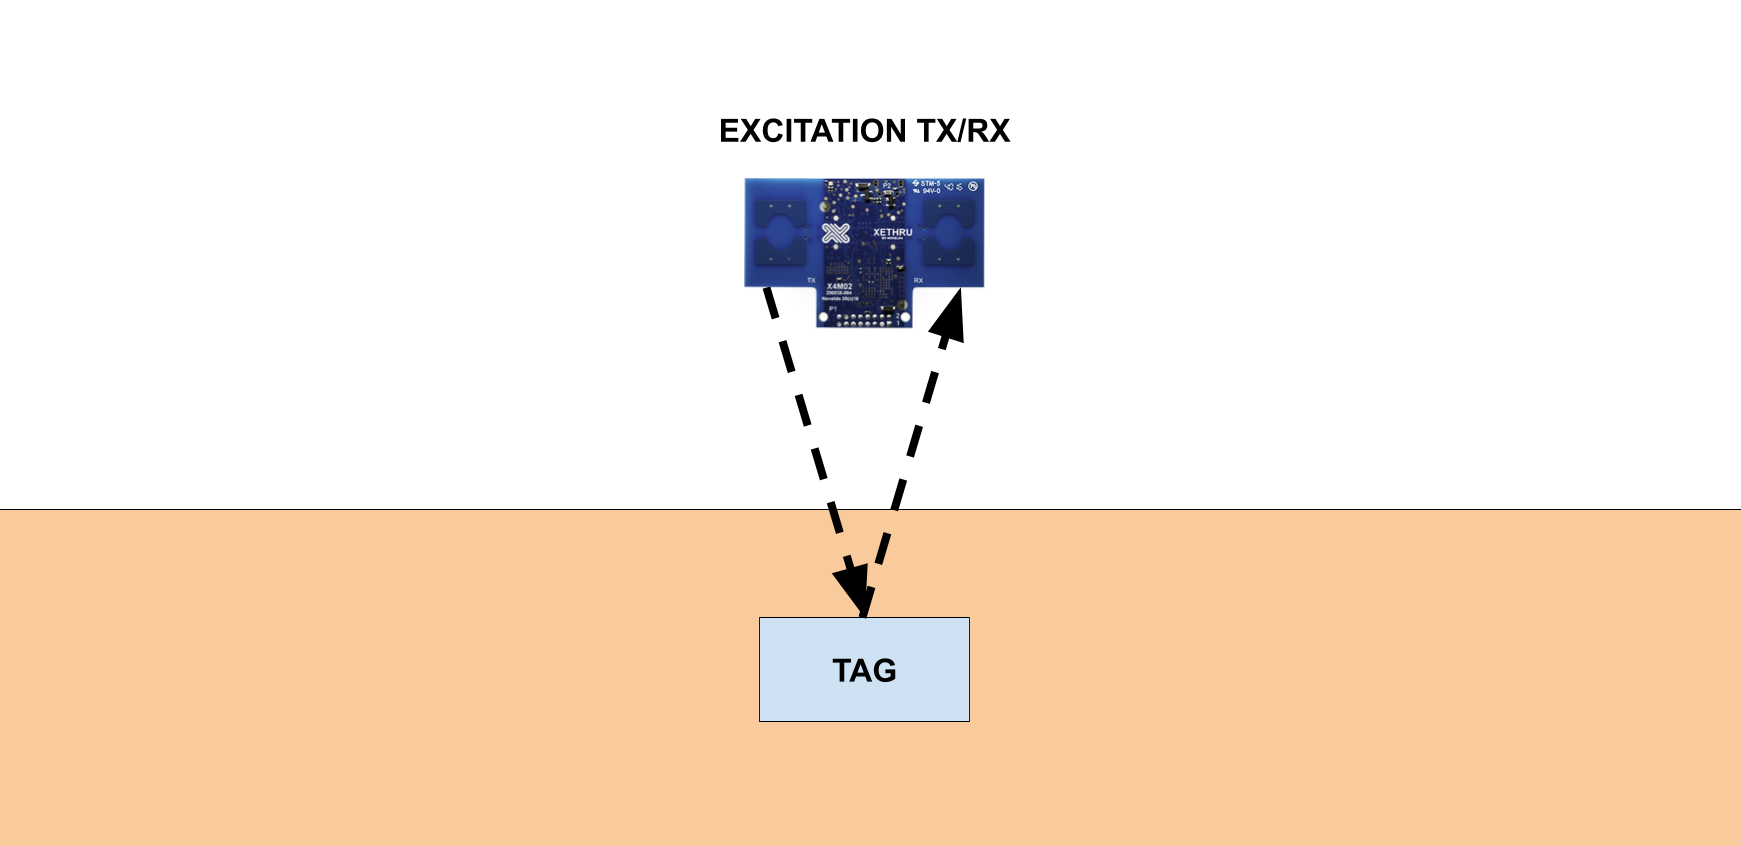
\includegraphics[scale=0.25]{soil_moisture_diagram.png}\\
  \caption{A potential UWB RADAR backscatter soil moisture sensing
    system}
\end{figure*}

Consumer-grade ultra-wideband Radars have the ability to accurately
measure the ToF of reflected signals. UWB radars typically have a
bandwidth of 2-7Ghz. This corresponds to a time resolution of
0.15-0.5ns. SMURF requires about 0.1ns ToF resolution. For
comparison, agricultural TDR sensors range from 100Mhz to
3Ghz~\cite{Pelletier2012} which leads to a resolution of at most
0.33ns. The ToF for a ranging radar is calculated by converting the
incoming samples back to the time domain and measuring the time delta
between peaks. Thus the sharper the peaks, the finer the possible time
resolution. A radar-based approach would have improved ToF resolution
by using the phase of the reflected signal in addition to the usual
ranging estimate technique. The time delta between the peaks would be
a coarse estimate, and the phase of the signal a fine tuning.

% The high bandwidth of the radars allows us to do a CDMA-inspired
% process introduced in ~\cite{}.

There are no commercially available backscatter tags currently
designed for use with radar, but fortunately the open-source design
for the HitchHike WiFi backscatter tags are compatible once the RF
switch is changed to match the bandwidth that the radar operates on.

One the tags are confirmed to be working with the radar above-ground,
the next key challenge will be burying the tags and discerning the
reflected backscatter signal from reflections due to the soil. One
possible approach is to toggle the backscatter tag at a relatively low
frequency, 100-500Hz. To the radar, this makes the tag look like it is
in motion, which makes the backscatter signal easy to pick out when
the rest of the environment is stationary. This clever approach was
designed by a labmate and is under review with no preprint. It is
discussed in detail in an appendix.

The ability to isolate the backscatter signal from other reflections
also has implications for how far the tags can be buried. The ideal
maximum depth would be 1+ meters, as crops that grow on trees often
benefit from moisture measurements at that depth. Depths of 10-30cm
are more than sufficient for a number of non-tree crops, though.

%% For the radar, a few low cost options are available. One is the
%% Walabot Developer UWB pulsed radar, which is readily commercially
%% available and has a bandwidth of 6.7Ghz. This corresponds to a ToF
%% resolution of 0.15ns. ~\cite{uwbThesis} shows that it is well suited
%% to being mounted on drones or autonomous robots for automated data
%% collection. This would allow both small-holder farmers and large
%% commercial farms to benefit. However, the frame rate supported by the
%% SDK may be too low. The documentation is sparse, so experiments are
%% needed.

%% The XeThru X4 radar series is another good option. The frame rate is
%% definitely sufficient to isolate a backscatter toggle between
%% 100-500hz, but the bandwidth is more narrow at 2.5Ghz. 

\section*{Preliminary results} 

We used an Analog Devices HMC1118LP3D switch evaluation kit, a 5-18
Ghz Vivaldi antenna from WA5VJB, and a teensy microcontroller that
acts as a programmable oscillators. The system is enclosed in a
locking plastic food storage box to provide water resistance. Future
prototypes will need to be fully waterproof.

\begin{figure}[h!]
  \centering
  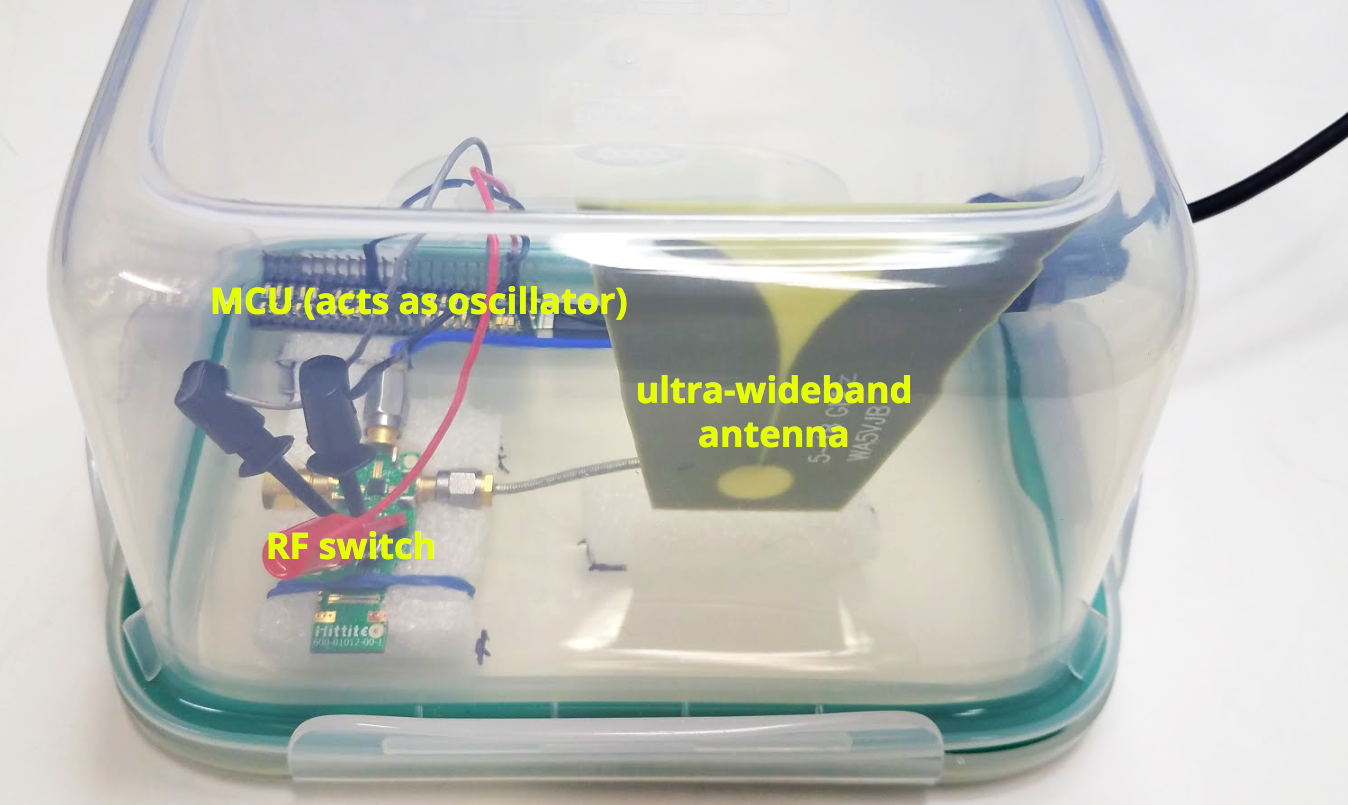
\includegraphics[scale=0.25]{prototype.png}\\
  \caption{An early water-resistant prototype of the backscatter tag}
  \label{figure:prototype}
\end{figure}

We used this tag plus a combination of Novelda XM03 and Flat Earth
Ancho/Cayenne/Chipotle radar development kits to perform preliminary
experiments on SNR vs tag depth and VWC estimations. 

The XM03 kit contains an X4 radar chip centered at 7.29GHz, the Ancho (X2)
is centered at 5.2Ghz, the Cayenne (X1) is centered at 4.3Ghz and the
Chipotle (X1) is centered at 1.5Ghz.

\subsection*{SNR vs depth}

We performed these experiments with the XM03, Ancho and Chipotle
radars. The Chipotle radar reaches a depth of 30cm ($\sim 1$ft), which is on
par with our minimum-viable depth goal. We need to repeat this
experiment for a variety of different soil wetness levels.

\begin{figure}[h!]
  \centering
  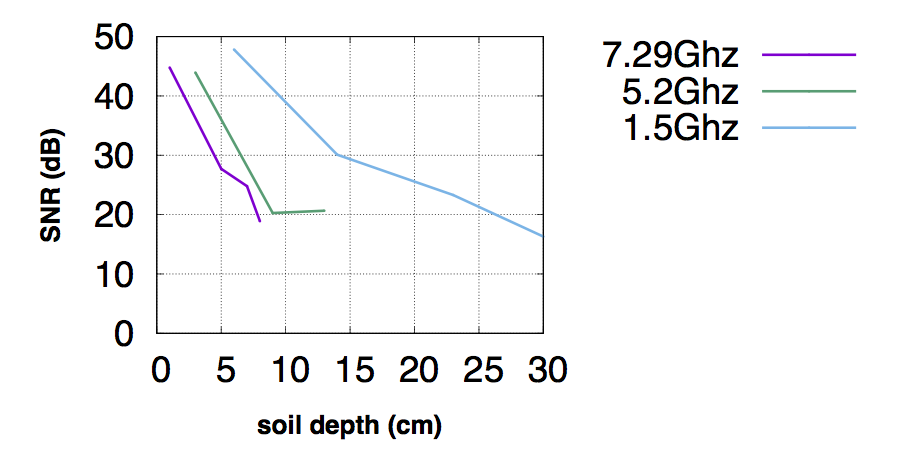
\includegraphics[scale=0.75]{../graphs/snr.png}\\
  \caption{SNR vs soil depth for 3 different radar center frequencies
    using damp potting soil.}
  \label{figure:depth}
\end{figure}

\subsection*{Soil moisture}

This experiment used the Cayenne radar, which is centered at 4.3Ghz.
The tag was buried at a depth of 7cm. The Cayenne has a small enough
range resolution ($\sim 4$mm) that we don't need to use phase
information to increase the ToF accuracy. However, due to the center
frequency it does not penetrate the soil as well as the Chipotle
radar. 

\begin{figure}[h!]
  \centering
  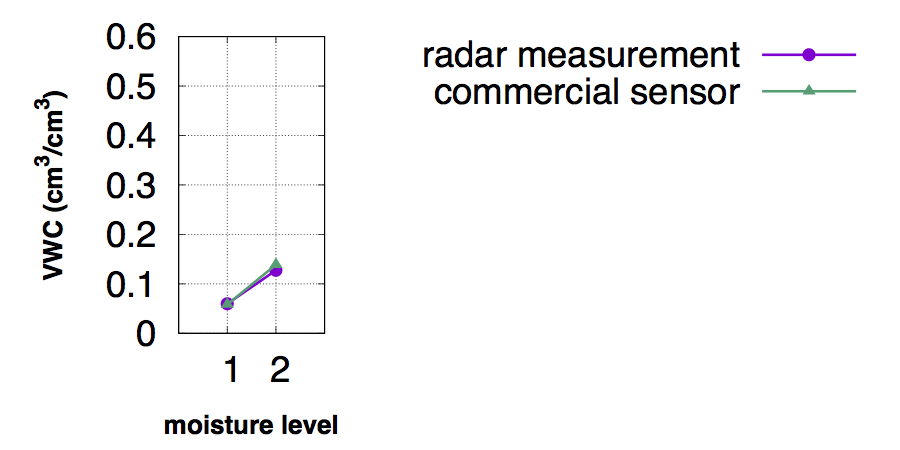
\includegraphics[scale=0.75]{../graphs/vwc.png}\\
  \caption{VWC was calculated using the Topp equation}
  \label{figure:moisture}
\end{figure}

We need to repeat this experiemnt with tag burried at 1ft,
which likely requires using the Chipotle radar. This radar has larger
range bins ($\sim 8$mm), so we would need to use phase data to get
accurate enough ToF. We also need to take more measurements on the
wetter side of the soil spectrum, up to saturation.

The average difference between the VWC calculated by our sensor and
the commercial sensor is 0.005$cm^3/cm^3$. This suggests that our
sensor is about as accurate as a commercial sensor. Though these
results are promising, we still need to compare them against a
ground-truth oven-based measurement. We also need to adapt our
calibrated equations to use the radar data so we can compare
calibrated results instead of just Topp equation results (currently
the calibrated equations are solved only for RAW Teros 12
measurements). Finally, we should perform the experiments on at least
one additional type of soil besides potting soil. We are planning to
collect soil from the Stanford Educational Farm, which is an
actively-producing vegetable and flower field located on
campus. Ideally we will also perform \emph{in sutu} measurements on
the field itself.

\section*{Next steps}

A core limitation we noticed during the preliminary experiments is
that the accuracy of the radar results depends heavily on how
accurately we can measure the depth of the soil on top of the tag. If
we can measure the depth to within about half a centemeter, the
results are good. Knowing the depth of the soil in this much detail is
feasible in a controlled environment, but it poses a major limitation
for use in a real farm field.

To avoid this problem, we can instead bury a sensor device that is
made of two or more tags separated vertically by a known distance (see
Fig.~\ref{figure:multiTag}). Then we can measure the absolute ToF for
each of the two tags and calculate the delta between the two. This
relative ToF allows us to estimate the moisture of the soil
\emph{between} the two tags. Because the distance between the tags is
fixed, only major changes to the soil environment will introduce
significant measurement error (e.g. flooding or tilling causing the
sensor to rotate or deform).


\begin{figure*}
  \hspace*{-0.8cm}
  \begin{minipage}[b]{0.55\textwidth}
    \centering
    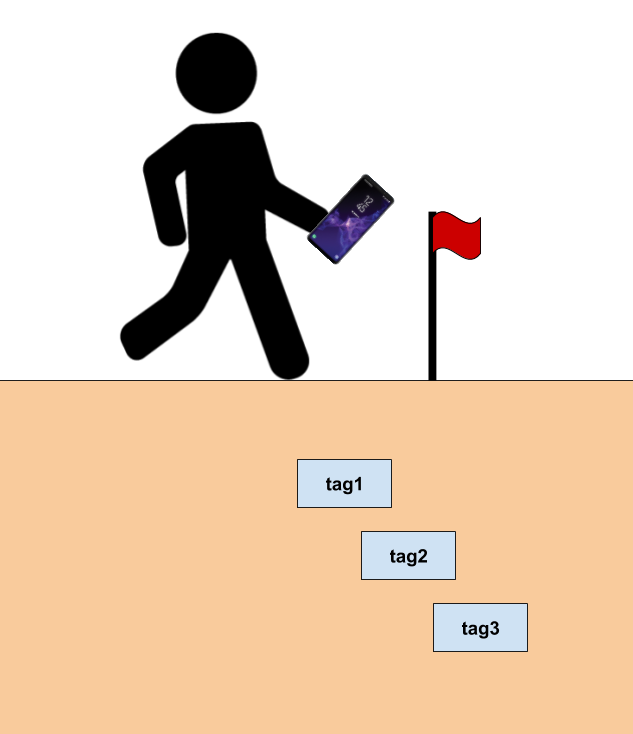
\includegraphics[scale=0.38]{multiTag.png}\\
    \subcaption{Overview of a system with three tags}
  \end{minipage}%                                                                                           
\begin{minipage}[b]{0.55\textwidth}
  \centering
  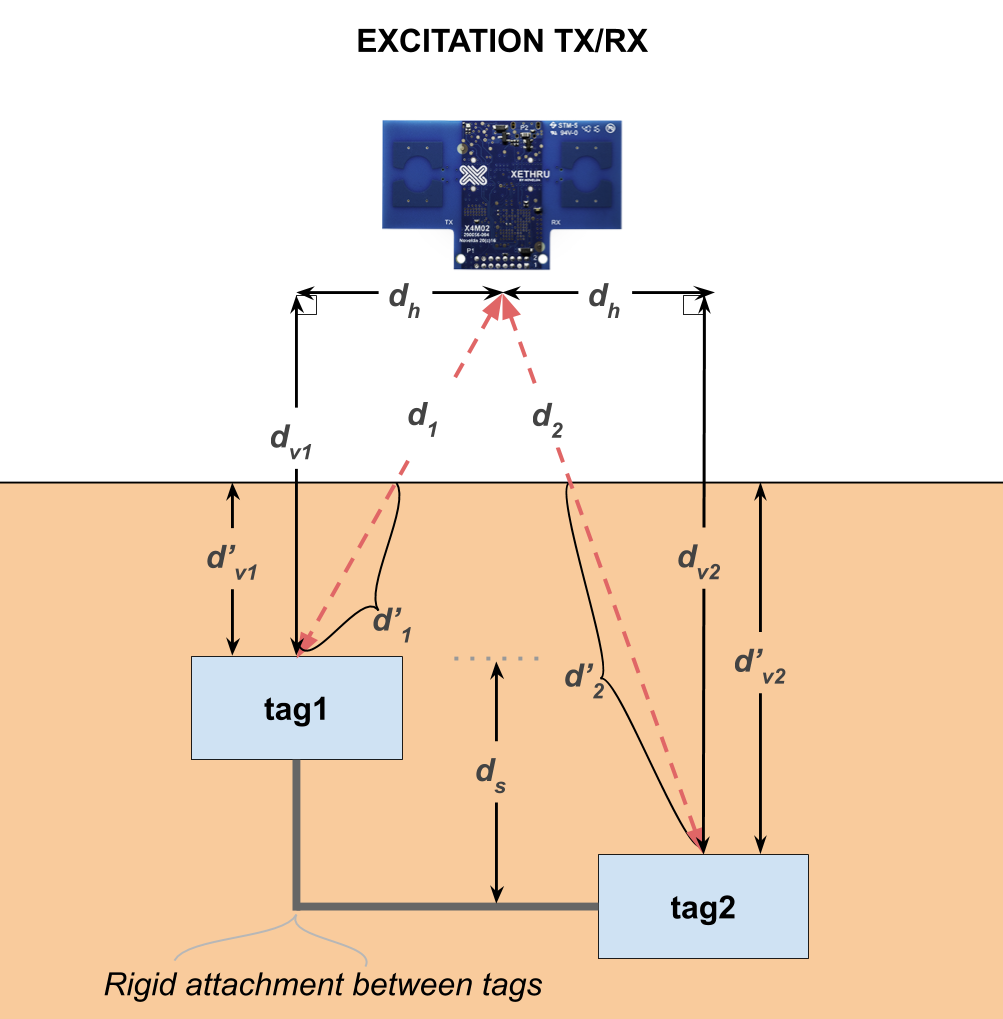
\includegraphics[scale=0.25]{multiTagCloseup.png}\\
  \subcaption{Close-up of proposed design with two tags}
\end{minipage}%                                                                                           
\caption{The proposed multi-tag system. In (a), the radar is connected
  to the farmer's smartphone for gathering measurements. In (b) two
  tags are rigidly attached, which keeps the inter-tag distances,
  $d_s$ and $d_h$ fixed.}
\label{figure:multiTag}
\end{figure*}


Unfortunately, we think our current prototype is too large for this
kind of setup. Because of how big it is, it will be difficult to
design a rigid attachmemt system for two of them, and they would also
not fit in our current indoors soil bins. Therefore we must choose
between three paths forward for the summer:

\begin{enumerate}
\item Continue taking measurements with the existing prototype and
  then fabricate the proposed two-tag system afterwards and redo the
  same experiemnts.
\begin{itemize}
\item Pros: 
\begin{itemize}
\item we will get important results sooner
\item if the preliminary results were a fluke, we can rethink our approach (fail fast)
\end{itemize}
\item Cons:
\begin{itemize}
\item the experiments will be more difficult to perform
\item duplicated work (two redundant sets of experiments, two
  different sets of software and hardware to debug)
\end{itemize}
\end{itemize}
\item Design and fabricate a PCB-based version of the prototype, then
  continue taking measurements.
\begin{itemize}
\item Pros:
\begin{itemize}
\item This will be the most impressive version of a prototype to submit
\item Only one set of experiments to perform
\item We will be able to relatively accurately predict the tag's useful lifetime
\end{itemize}
\item Cons:
\begin{itemize}
\item None of the authors have ever fabricated a PCB before
\item The oscillation frequencies of the tag will need to be frozen
\item PCB is more difficult to debug
\end{itemize}
\end{itemize}
\item Design a new stopgap prototype that uses a wideband chip antenna
  instead of the Vivaldi antenna, then continue taking measurements.
\begin{itemize}
\item Pros: 
\begin{itemize}
\item Only one set of experiments to perform
\item Using a chip antenna will more accurately reflect the performance of any eventual product
\item The time investment for this design is (probably significantly) less than designing a PCB
\item We will probably need to evaluate the efficacy of chip antennas and waterproof enclosures before submitting a PCB design anyway
\end{itemize}
\item Cons: 
\begin{itemize}
\item if the preliminary results were a fluke, we will have wasted some time building this prototype
\end{itemize}
\end{itemize}
\end{enumerate}

The final approach is the most promising, because it allows us to test
the two-tag system soonest and also at low cost (no PCB manufacuring
run necessary). Furthermore, instead of struggling to do absolute ToF
measurements, I believe we can simply use the relative phases between
the tags. However, we may need to calculate and compensate for
hardward-specific offsets\footnote{How noticable does the offset have
  to be before we need to compensate for it? How fixed is the offset
  (how strong is the dependence on environmental factors like
  temperature? can we calibrate once per tag? can we calibrate once
  and apply the same compensation to any tags using the same
  design?}. Therefore we propose the following schedule:

\begin{itemize}
\item July 1-14:
  \begin{itemize}
  \item Get data for SNR vs soil moisture with Chipotle and tag buried 1
    ft (REUs can do this)
  \item Work with antenna experts to find an appropriate small
    form-factor antenna. Will likely need to be custom.
  \item Purchase an appropriately sized waterproof enclosure and
    figure out how to rigidly attach two of them
  \item Using existing antennas, accurately measure relative ToF in
    open air using Chipotle (X1 1.5Ghz) phase
  \end{itemize}
  
\item July 15-28:
  \begin{itemize}
  \item Conduct soil moisture experiments with revised prototype,
    measuring permittivity and comparing against commercial sensor and
    oven (REUs can help with this)
  \item Calibrate Teros sensor on Farm soil (REUs could do this)
  \item Redo moisture experiments with Farm soil (this may extend into
    August depending on how long making the new prototypes takes)
\end{itemize}

\item August
\begin{itemize}
\item Quantify anticipated tag battery life.
\item Do in-situ measurements on Farm
\item Write Mobicom or NSDI research paper
\end{itemize}
\item September: present results at MSR
\end{itemize}

\section*{Future work}
\subsubsection*{Electrical Conductivity} It might also be possible for a
backscatter system to measure electrical conductivity (EC), which is
another parameter that soil moisture sensors sometimes measure. EC is
related to the salinity of the soil and is correlated strongly with
crop health.

\subsubsection*{Calibration} One current weakness with all sensors is the
need to calibrate them to specific soil types. Is it possible to set
easy-to-follow guidelines, or even to automatically detect and
calibrate for the soil type? This would massively decrease the
deployment and usage barriers.

\subsubsection*{Environmental impact of tags}
How readily do the tags get detached and lost in the soil? How does
this impact the growing environment, especially if the tags use
batteries?

\subsubsection*{Leaf moisture}
Leaf moisture or leaf thickness is a more reliable measure of how much
water a plant needs, but it is significantly more difficult to collect
than soil moisture. The sensors without data loggers and
communications are \$300 and are unwieldy and
delicate. ~\cite{Wang2017} uses RFID tags to identify and measure
liquids, and can even tell the difference between a vessel containing
Coke and Pepsi. Could this be extended to measuring the leaf thickness
or nutrient absorption of plants?


\section*{Conclusion}
Technology in agriculture is a relatively unexplored area, especially
within the academic EE and communications communities. This creates
opportunities for cross-disciplinary work and opens up a rich set of
open problems with global impact. Using RF backscatter to detect
soil moisture is an interesting and useful application of backscatter
and radar technologies, with multiple potential future works. We
believe it will address the shortcomings of present sensing solutions,
and will also be accessible to small and large farms alike.

\bibliographystyle{amsplain}
\begin{footnotesize}
  \bibliography{soilProgress}
\end{footnotesize}

\section*{Appendix: Radar}
RADAR (RAdio Detection And Ranging) is a well-developed technology
with a history dating back to before World War II. Conceptually
similar to echolocation, it uses the Time of Flight and angle of
arrival of RF waves to calculate the distance of objects and their
speed.

Radar was originally used primarily in military contexts, but nowadays
it is used to predict weather patterns, measure the speed of vehicles
and other objects, assist autonomous vehicle navigation, and even
monitoring human breathing.

There are two primary types of radar waveforms: continuous wave and
pulsed~\cite{Richards2010}. Continuous wave radars are transmitting
and receiving at all times, while pulsed radars periodically transmit a
short-duration pulse and listen for the reflections to come back.

The most basic types of continuous wave radar use the Doppler shift of
moving targets to calculate their speed, and they are incapable of
calculating the target distance, or \emph{range}. Frequency Modulated
Continuous Wave (FMCW) is a variant that is capable of calculating
range as well as speed. It periodically sweeps the transmit signal
through a frequency range, and measures the frequency delta between
the transmitted and received signal to calculate distance.

Pulsed radars\footnote{Pulse radars are also sometimes called
  pulse-Doppler radars because they Doppler to measure the speed of
  targets. Confusingly, basic CW radars are sometimes just called
  Doppler radars because they too use Doppler to measure speed.} can
very easily determine the range of a target by measuring the time that
elapses between pulse transmission and the return reflection. They can
also measure target speed. When the pulse width of the radar is very
short, it is known as an impulse radar or Ultra Wideband (UWB)
radar. UWB radars were enabled by a key circuits discovery in 1994:
the single-shot transient digitizer~\cite{}. This device is capable of
high speed, high accuracy digitization of very short pulses of enegry
(< 5ns). This allowed for the construction of a significantly cheaper
and smaller radar transceiver that digitizes incoming RF and
correlates it with the transmitted pulse samples. 

Impulse radar needs to be wideband because of Fourier duality:
pulses that are short in the time domain require wide bandwidth in the
frequency domain. The bandwidth of a UWB radar typically ranges
between 2 and 8 Ghz. Furthermore, the transmit power of UWB radars is
usually regulated to be very low to avoid causing interference to
other users on the same spectrum. This also makes UWB radar very
difficult to detect, as the transmitted waveform looks like white
noise. UWB radars are also popular because the low transmission power
ensures that the signal is harmless to humans. The transmit power
regulations also restrict the operating range of UWB radars to
relatively short distances, typically $<25$m for consumer grade
radars.

%% \begin{figure*}[h!]
%%   \centering
%%   \includegraphics[scale=0.5]{radarDiagram.png}\\
%%   \caption{Transceiver of the X4 radar~\cite{X4datasheet}}
%%   \label{fig:radarDiagram}
%% \end{figure*}

%% Figure~\ref{fig:radarDiagram} is a diagram of the X4 impulse radar
%% transceiver. 

A modern radar operates using \emph{frames}, which is the set of
samples from a single sweep across the radar's sensing area. Once
converted to baseband, the frame has one complex sample per
\emph{range bin}. Each range bin corresponds to a range of possible
distances from the radar. For example, if the radar resolution is 5cm,
the magnitude of the sample from the 10th range bin would correspond
to an object that is 45-50cm away from the radar.

\subsubsection*{Signal processing}

Let the transmitted impulse be represented by $p(t)$, and the received
sigal by $r(t)$. Then, digitized sample for the $n$th range bin can be
written as

\begin{equation}
r[n] = \alpha p(nT - \tau)  
\end{equation}

Where $T$ is the sampling period\footnote{this is also the duration of
  the transmitted impulse}, $\alpha$ is the complex attenuation and
$d_k$ is the distance of the range bin in meters. Time of flight,
$\tau_k = 2d_k/c$, is the time for a radar impulse to travel to an object and
then reflect back again. 

For simplicity we have assumed that there is only one reflector per
range bin, but in reality there are multiple reflections in a range
bin. Then the resulting sample will be the linear combination of the
$k$ reflectors:

\begin{equation}
r[n] = \sum\limits_{k=1}^K \alpha_k p(nT - \tau_k)  
\end{equation}

Because pulse-based radars transmit at a regular interval (known as a
PRI), they can be used to obtain the speed of moving objects. If an
object is moving at a constant speed of $v$ m/s, then every frame the
time of flight changes by $2v\Delta/c$ where $\Delta$ is the PRI.

This change in the time-domain ToF corresponds to a change in phase in
the frequency domain: $\phi_k = 2\pi f (2v_k\Delta/c)$. Although the
phase changes for each frequency within the bandwidth of the impulse,
we can simplify the math by using only the radar's center frequency
$f_c$\footnote{This approximation is only valid for signals where the
  bandwidth of the signal is small compared to the center
  frequency. The X4 has a 2Ghz bandwidth centered at 8Ghz, so this
  assumption is somewhat valid but may not be for other radars. I
  asked Dustin Schroeder about this issue, and he suggests that pulse
  compression takes care of this issue.}. Then, the value for the
$n$th bin in the $m$th frame will be


\begin{equation}
r_m[n] =  \sum\limits_{k=1}^K \alpha_k p(nT - \tau_k)e^{-j2\pi  \frac{2 v_k \Delta(m-1)}{\lambda}}  
\label{eq:timedomain}
\end{equation}

where $\lambda$ is the wavelength of the radar center frequency,
$f_c$.

Note how similar Eq.~\ref{eq:timedomain} is to the discrete Fourier transform,

\begin{equation}
F_k = \sum\limits_{k=1}^{N-1} f_n e^{\frac{-j2\pi}{N}kn}
\end{equation}

If we apply a 1-D inverse Fourier transform to each range bin across a
collection of P pulses, we get a \emph{range-Doppler image} which
tells us the speed of moving objects:

\begin{equation}
R[n,s] = \sum\limits_{i=1}^{P} r_m[n] e^{-j2\pi\frac{(i-1)(s-1)}{P}}
\label{eq:rangedopp}
\end{equation}

In Eq.~\ref{eq:rangedopp} above, $s$ is the Doppler bin and $n$ is
the range bin and $P$ is the total number of pulses transmitted over
the collection time. 

\begin{figure}[h!]
  \centering
  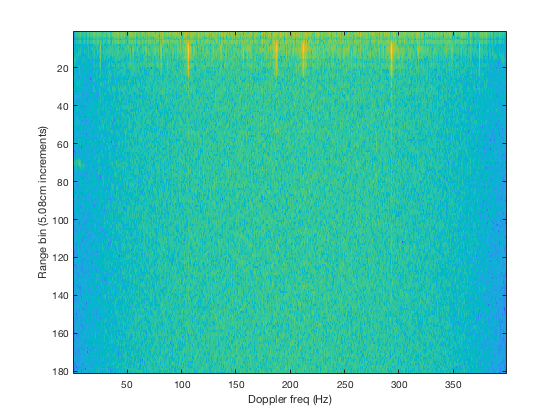
\includegraphics[scale=0.5]{rangedoppler.png}\\
  \caption{A range-Doppler image generated from an X4 radar capture}
  \label{figure:rdplot}
\end{figure}

Figure~\ref{figure:rdplot} shows an example range-Doppler plot. We can
see that there are bright spots at 212 and 293 Hz. This plot is a 10
second capture where the radar is pointed at antennas that are
grounded and ungrounded at those frequencies. If there are no other
fast-moving objects in the radar's field of view, we can use this
property to discern the signal from our backscatter tag from the
signals due to other reflectors.

We simply use the built-in FFT function of MATLAB, but there are a
number of more sophisticated techniques to improve results. More
details on range-Doppler formation can be found
in~\cite{rangeDoppler}.

\subsubsection*{Signal attenuation}

Another key challenge with radar backscatter is signal
attenuation. Higher frequency RF has difficulty passing through RF, so
when the soil is wet how deep can the tag be before we lose the
signal?

The \emph{dynamic range} of an analog to digital converter (ADC) is
how many quantization bins there are. The X4 radar has an 11-bit ADC,
which corresponds to 66dB. The automatic gain control (AGC) amplifies
the incoming signal until the peak value is in the maximum
quantization bin. The largest signal component will be the
\emph{leakage} from the TX to RX of the radar, which corresponds
roughly to the signal magnitude in the 0th bin. If the AGC multiplies
the incoming signal by $N$, then the backscatter signal needs to be at
least $1/N$ of the quantization unit in an ideal case (no noise). If
there is noise, then the signal needs to be one bin louder.

Then, knowing this minimum volume we could use the penetration depth
(or a related metric, path loss) to estimate the maximum
depth. Penetration depth measures how deep electromagnetic radiation
can penetrate into a material. It is defined as the depth at which the
intensity of the radiation inside the material falls to $1/e$ (about
37\%) of its original value at the surface. The penetration depth
depends on the center frequency, and it is typically found in
lookup-tables. Unfortunately, the penetration depth of damp soil is
not well studied. There is one ITU study that has penetration depths
of wet and dry soil as a function of
frequency~\cite{penetrationDepth}, but they do not provide details on
the soil type or moisture level(s).

Path loss, $L$, is the reduction in power density (attenuation) of an
electromagnetic wave as it propagates through space. Linear path loss
is the ratio of transmit power to receive power~\cite{goldsmith}. Path
loss is the linear path loss expressed in dB. In the simplified path
loss model, a material or environment is associated with a \emph{path
  loss exponent}, $\gamma$:

\begin{equation}
  L = 10\log_{10}(d)^\gamma + C
\end{equation}

In the equation above, $d$ is the distance between the TX and RX in
meters and $C$ is a constant accounting for things like antenna
characteristics. Path loss values typically range from 2-6, with 2
being the path loss of free space. Like penetration depth, the path
loss of soil is also not well studied. However, we expect that the
loss for damp soil will be significantly higher than 6.

Given how inexact our knowledge is of the path loss and/or penetration
depth of potting soil, these bounds are not especially
useful. Therefore our approach was to experimentally determine SNR vs
soil depth for various moisture levels. 

\subsection*{SNR}

keith says to anticipate a question about how the accuracy of the soil
sensor measurement will depend on the SNR

Range measuring error is inversely proportional to the square root of
the SNR, so the lower the SNR the higher the error will be. However,
the measurement error is also proportional to the range bin so the
smaller the range bins the smaller the error. The range bins in our
radar are pretty small, they correspond to 1/10 to 1/20 ns, which is
equivalent to about 0.01-0.03cm3/cm3 in VWC ambiguity (again
comparable to a commercial sensor). In short, the smaller the range
bins the more tolerance the system has for low SNRs.


\subsubsection*{Improving SNR}
Given the low-SNR nature of backscatter, it is worth investigating
radar configurations and post-processing techniques that can improve
our SNR.

Different models of radar have different receive chains, which
informs how the signal is digitized and what the operator can do to to
isolate weak signals. The receive chain has an LNA followed by a
sampling/ADC system. The X4 radar (and possibly the X2) uses a
technique called Swept Threshold sampling~\cite{sweptThreshold}. Most
models of radar let the user adjust the DAC settings, which impacts
the maximum and minimum accepted input voltage, and also the
quantization step size. Having low DAC mins and maxes with a small
quantization step size may allow us to target low-SNR signals.

As far as post-processing, a few UWB radar applications use SVD-based
clutter removal to improve the signal strength
~\cite{uw~bRange}~\cite{svdClutter}. These techniques may be worth
investigating.

\section*{Signal processing}
The output of the X1 and X2 radars for a single frame is N doubles,
where N is the number of samplers that the radar contains. These data are
modulated RF samples, centered around the radar carrier center frequency
$f_c$.

The unmodulated data are centered around zero and called
\emph{baseband} samples. One common way of modulating signals is to
vary the amplitude of phase-shifted sinusoids that are oscillating at
the carrier frequency. If the phase difference between two sinusoids
is 90 degrees ($\pi/2$ radians), (e.g. the sine and cosine wave), then
these two signals are said to be in quadrature. Conventionally, cosine
is considered to be \emph{in phase}, or I, and sine is
\emph{quadrature phase}, or Q. I represents the amplitude of the
in-phase component of a baseband singal, and Q is the amplitude of the
quadrature phase component.

\subsection*{Digital downconversion}
Digital downconversion is the process of converting received RF
singals back down to baseband. It has three steps:

\begin{enumerate}
\item frequency shifting the RF signal
\item filtering the shifted signal
\item (optionally) downsampling the data 

The frequency shifting is done by mixing the RF signal with local
oscillator (LO) signals in quadrature, i.e. multiplying the the
samples by sine and cosine oscillating at the carrier
frequency. Conventionally, this turns the real-valued RF sample into a
complex number with the real-part being the in-phase I component and
the complex part being the quadtarture-phase Q component:

\begin{equation*}
b = s(cos(2\pi f_c t)+ jsin(2 \pi f_c t)) 
\end{equation*}

\end{enumerate}


\section*{Soil equations}
Time of flight, $\tau$, meaures the \emph{apparent dielectric
  constant} $K_a$, which is a function of
$\varepsilon_r', \varepsilon_r'', \varepsilon_0$ and electical conductivity (EC)
$\sigma$:

\begin{equation}
  K_a = \frac{\varepsilon_r'}{2}\Bigg[\sqrt{1+\bigg(\frac{\varepsilon_r'' + \frac{\sigma}{2\pi f\varepsilon_0}}{\varepsilon_r'}\bigg)^2}+1\Bigg]  
\end{equation}

At high frequencies, $\epsilon_r$ is dominated by the real part
$\epsilon_r'$, so $K_a$ approximates $\epsilon_r'$. Then we have

\begin{equation}
K_a \approx (\frac{c\tau}{d})^2
\end{equation}

where $c$ is the speed of light and $d$ is the known distance (in
meters) that we calculate the ToF for.

Soil moisture $\Theta$ can be related to $K_a$ using formulas that depend on the soil type. One such formula is the Topp Equation ~\cite{Topp1980}, which is applicable to ``average soils'':

\begin{equation}
  \Theta = 4.3\times 10^{-6}K_a^3-5.5\times10^{-4}K_a^2+2.92\times 10^{-2}K_a-5.3\times 10^{-2}
\end{equation}

Where the units of soil moisture are $cm^3/cm^3$. This the ratio of water volume over dry soil volume.

Substituting,

\begin{equation}
  \Theta \approx 4.3\times 10^{-6} (\frac{c\tau}{d})^6-5.5\times10^{-4} (\frac{c\tau}{d})^4+2.92\times 10^{-2} (\frac{c\tau}{d})^2-5.3\times 10^{-2}
\end{equation}

To be on par with commercial soil sensors, we want our soil moisture
measurements to be within $0.05 cm^3/cm^3$ of the actual soil moisture
(measured with an oven). This also means we need a resolution of at
least $0.05 cm^3/cm^3$.

Waves slow down 2-6 times in soil compared to the speed of
light~\cite{gpr}. Assuming a distance of 1m and a slowdown of 3x,
$\tau = 10.006$ns. Then,

\begin{equation}
  \Theta \approx 3.1\times 10^{45}\tau^6-4.44\times 10^{30}\tau^4+2.6\times 10^{15}\tau^2-0.053 = 0.1657
\end{equation}

Referring to Table 1, With a ToF resolution of 1ns, we will get a
delta of $0.035-0.04 cm^3/cm^3$, which is within our bounds. However,
the equation is nonlinear, so a smaller ToF delta is helpful. If we
achieve 0.1ns, the resulting VWC resolution is about 0.003-0.004. Of
course, just because we have the necessary resolution does not mean
our sensor will be accurate within 0.05$cm^3/cm^3$.


\begin{table}[]
  \centering
\begin{tabular}{l|l}
\textbf{ToF (ns)} & \textbf{VWC ($cm^3/cm^3$)} \\ \hline
9.0               & 0.1301                                                      \\
9.9              & 0.1620                                                       \\
  10.0              & 0.1657                                                       \\
10.1              & 0.1693                                                       \\
11.0              & 0.2020                                                      
\end{tabular}
\end{table}

\subsection*{Calibrations}
During winter 2019 we performed calibration method B (specified in the
Teros 12 manual) on Vigoro potting soil. Figure~\ref{figure:calib}
shows that our custom calibration more closely tracks the actual
volumetric soil moisture (measured with an oven). The average error
for the Meter-supplied spotting soil equation is $0.066 cm^3/cm^3$,
which is actually more than twice the manual's claimed accuracy for a
generic caibration ($0.03 cm^3/cm^3$). However, our custom calibration
has an error of $0.29cm^3/cm^3$, which is much better.

\begin{figure*}[h!]
  \centering
  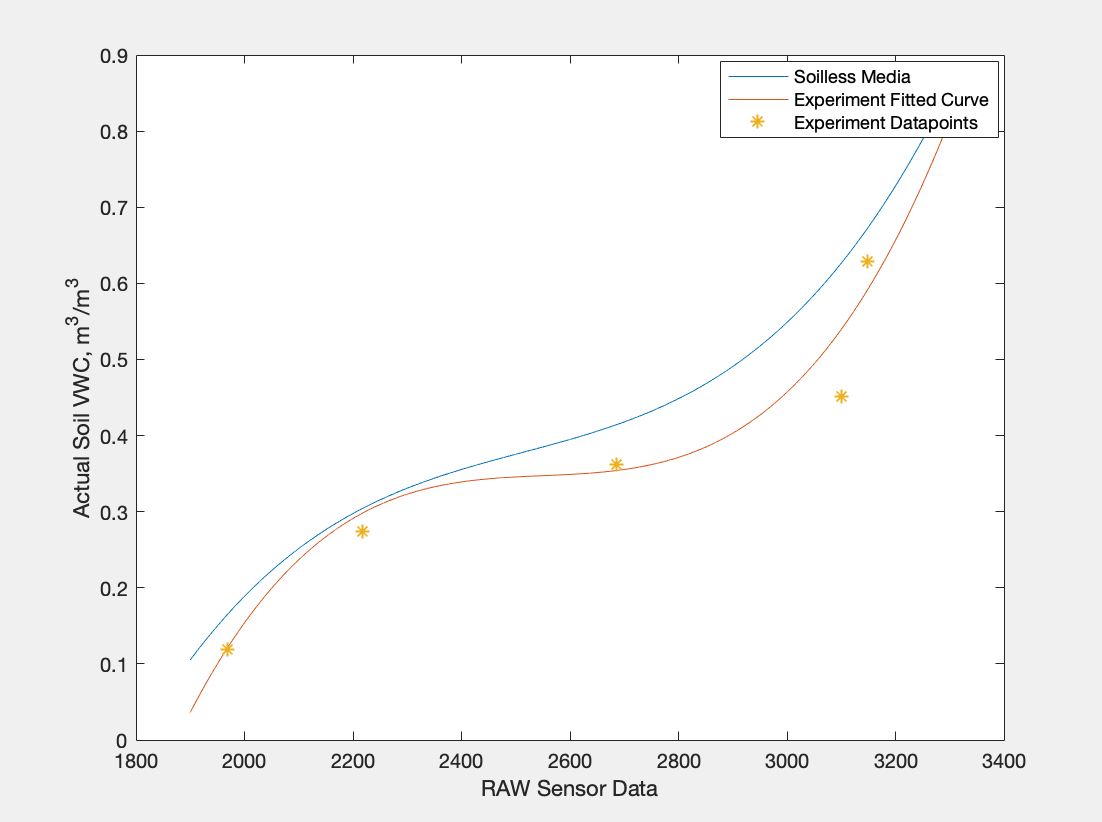
\includegraphics[scale=0.8]{teros12calib.png}\\
  \caption{A comparison of the Meter-supplied potting soil equation vs our custom calibration}
  \label{figure:calib}
\end{figure*}


\subsubsection*{Custom calibration equation:}
\begin{equation*}
\theta = (1.059\times 10^{-9})RAW^3 - (8.088\times 10^{-6})RAW^2 + (2.066\times 10^{-2})RAW - 17.27
\end{equation*}

Where $RAW$ is the raw Teros 12 sensor reading for soil moisture

\subsubsection*{Meter soilless media (e.g. potting soil) equation:}
\begin{equation*}
\theta =   (6.771\times 10^{-10})RAW^3 - (5.105\times 10^{-6})RAW^2 + (1.302\times 10^{-2})RAW - 10.848
\end{equation*}

\end{document}
